%----------------------------------------------------------------------------------------
%	PACKAGES AND THEMES
%----------------------------------------------------------------------------------------
\documentclass[aspectratio=169,xcolor=dvipsnames]{beamer}
\usetheme{SimplePlus}

\usepackage{amsmath}

%\usepackage[T1]{fontenc}
\usepackage[utf8]{inputenc}
\usepackage[serbian]{babel}

%\usepackage[T1]{fontenc}

\usepackage{hyperref}
\usepackage{graphicx} % Allows including images
\usepackage{booktabs} % Allows the use of \toprule, \midrule and \bottomrule in tables

%----------------------------------------------------------------------------------------
%	TITLE PAGE
%----------------------------------------------------------------------------------------

\title[short title]{Upravljanje brzinom motora jednosmerne struje primenom analogne negativne povratne sprege} % The short title appears at the bottom of every slide, the full title is only on the title page
\subtitle{Diplomski rad}


\author {Mentor: Prof. Dr Radivoje Đurić
\qquad\qquad
\hfill Kandidat: David Milovanović
}


\institute[NTU] % Your institution as it will appear on the bottom of every slide, may be shorthand to save space
{
    Univerzitet u Beogradu \\
    Elektrotehnički fakultet % Your institution for the title page
}
\date{\today} % Date, can be changed to a custom date
%\date{28. septembar, 2022}


%----------------------------------------------------------------------------------------
%	PRESENTATION SLIDES
%----------------------------------------------------------------------------------------

\begin{document}

\begin{frame}
    % Print the title page as the first slide
    \titlepage
\end{frame}

\begin{frame}{Pregled}
    % Throughout your presentation, if you choose to use \section{} and \subsection{} commands, these will automatically be printed on this slide as an overview of your presentation
    \tableofcontents
\end{frame}

%------------------------------------------------
\section{Teorijski uvod}
%------------------------------------------------

\begin{frame}
    \Huge{\centerline{\textbf{Teorijski uvod}}}
\end{frame}
%------------------------------------------------


\subsection{Sistemi automatskog upravljanja}

\begin{frame}{Sistemi automatskog upravljanja}
    \begin{figure}
    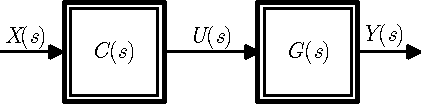
\includegraphics[width=0.6\linewidth]{fig/sau.pdf}
    \caption{Opšta blok šema sistema automatskog upravljanja.}
    \end{figure}
\end{frame}

%------------------------------------------------
\subsection{Motor stalne struje}

\begin{frame}{Motor stalne struje}
	\begin{columns}[c]
    \begin{column}{.5\textwidth}
    \begin{figure}
        \centering
        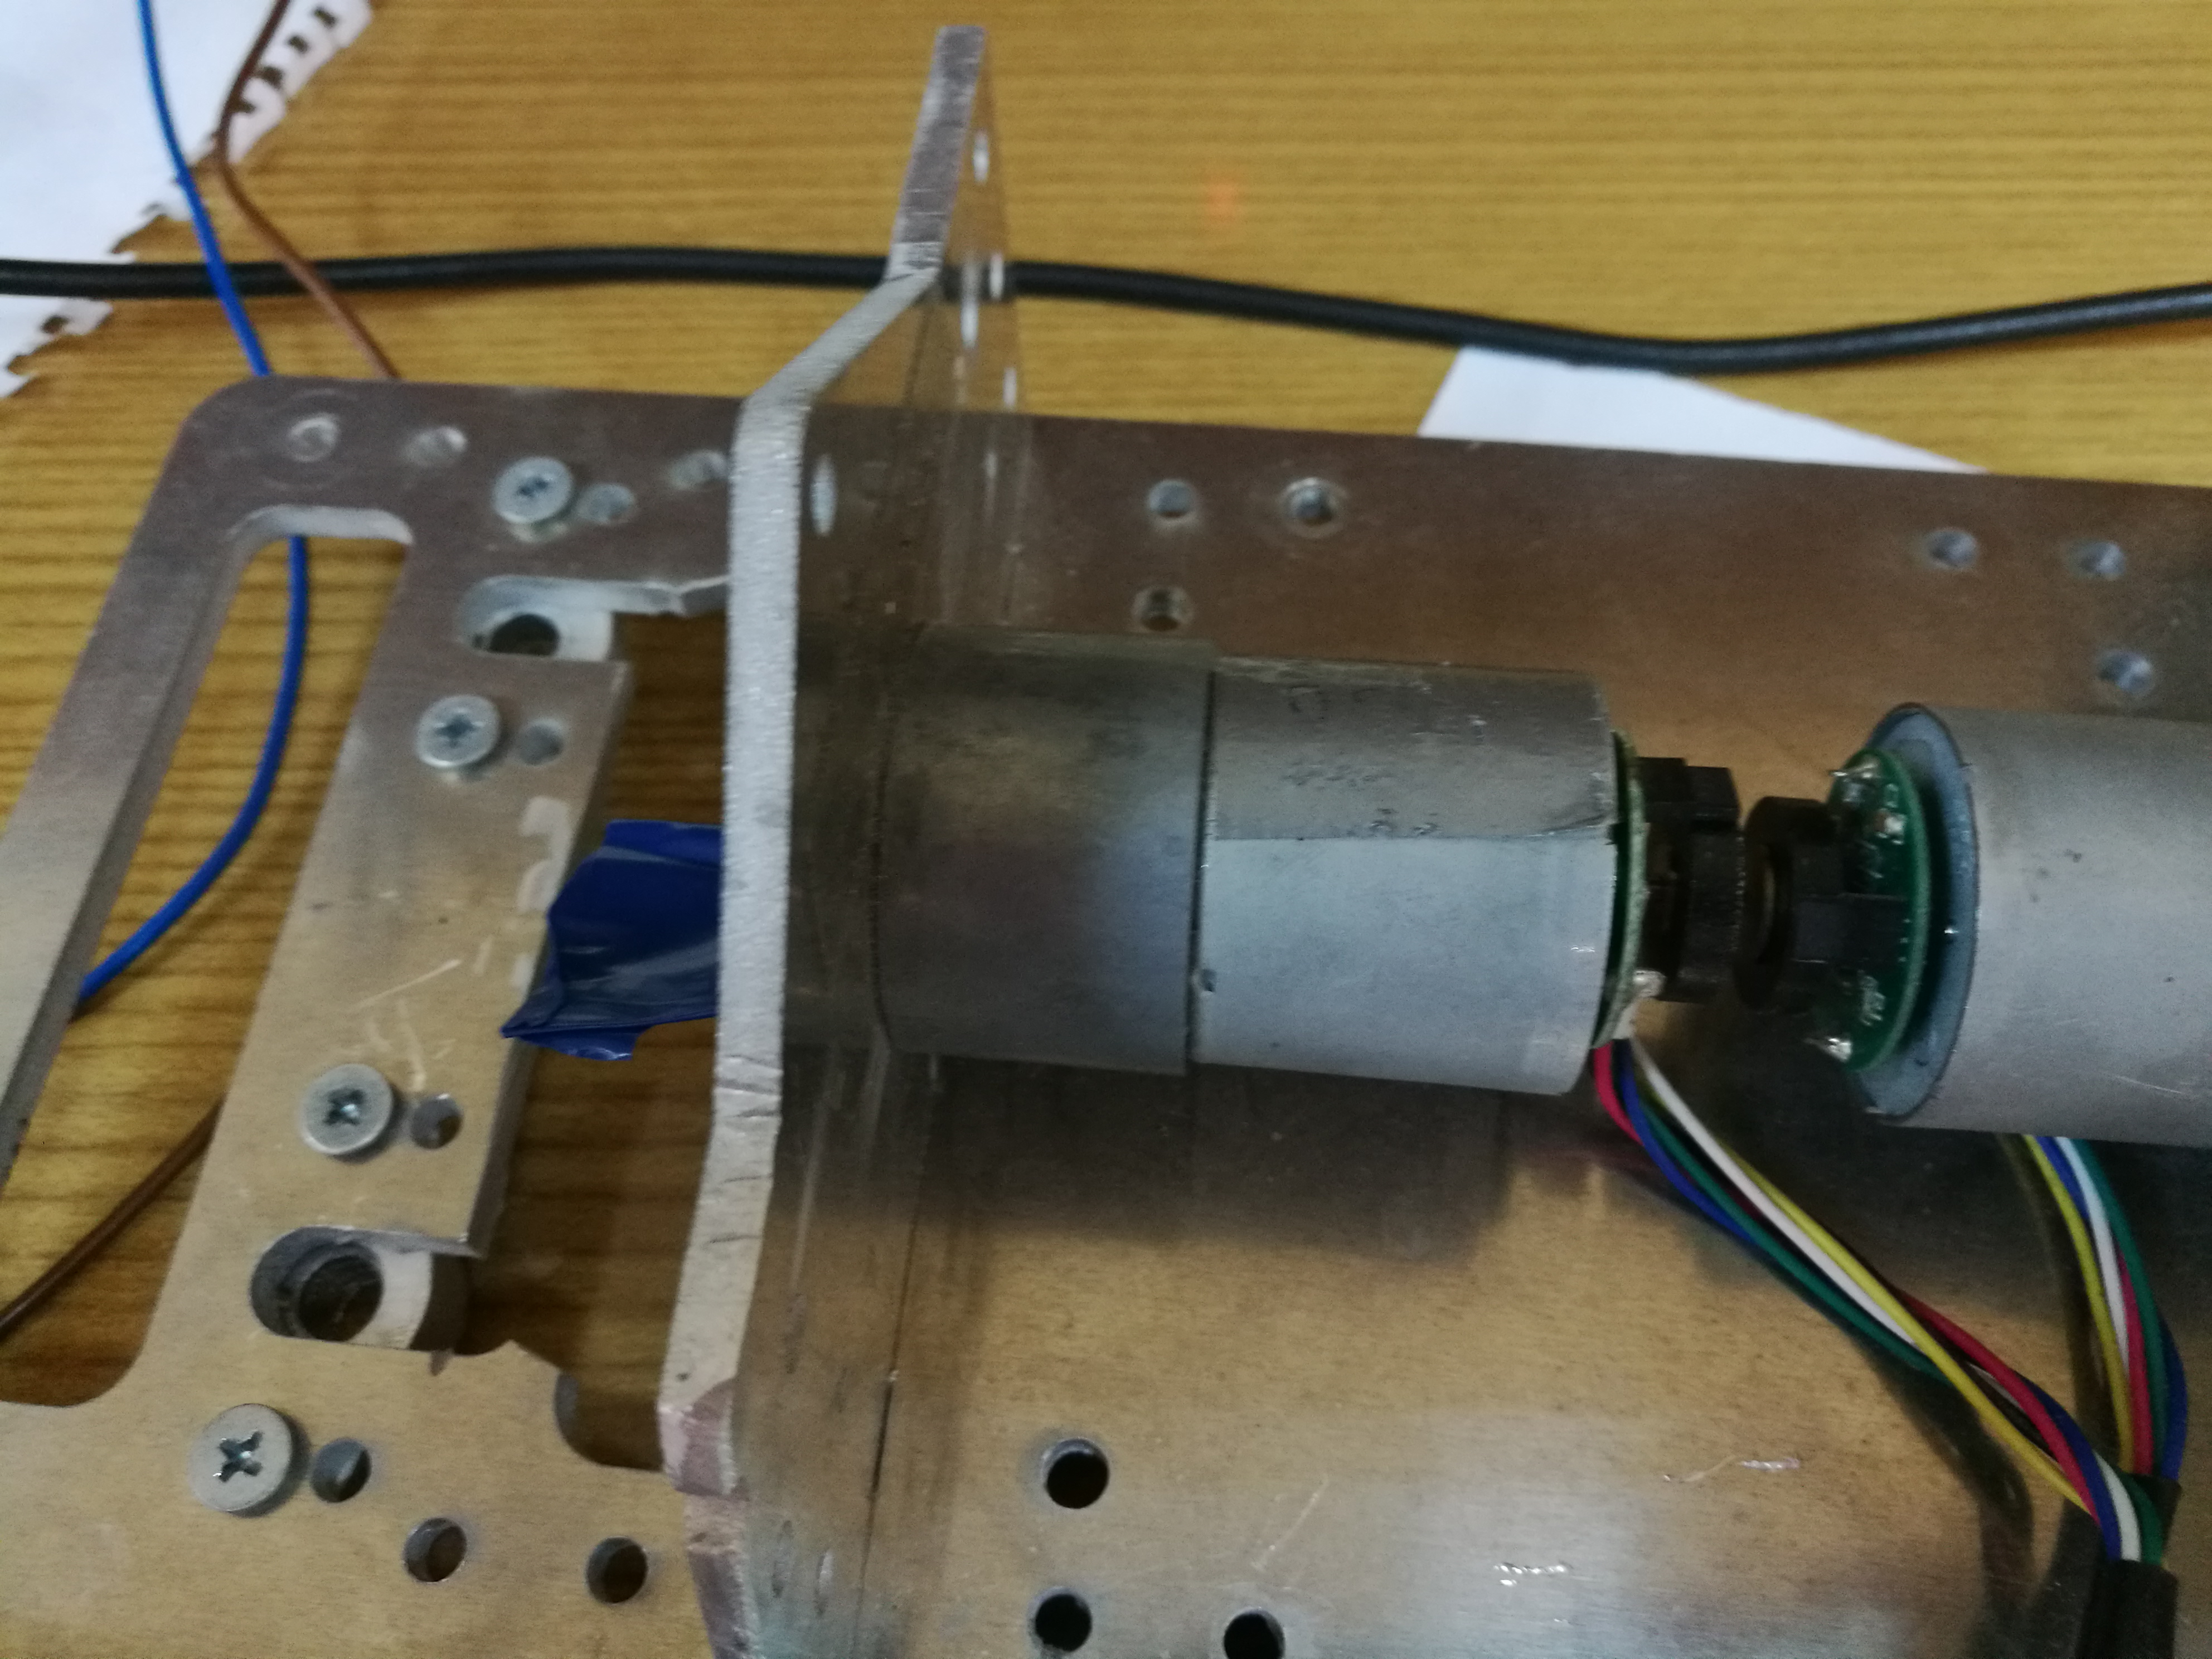
\includegraphics[width=0.8\textwidth]{fig/DCmotor.jpg}
        \caption{Motor stalne struje.}
    \end{figure}      
    \end{column}
    \begin{column}{.5\textwidth}
    \begin{figure}
        \centering
        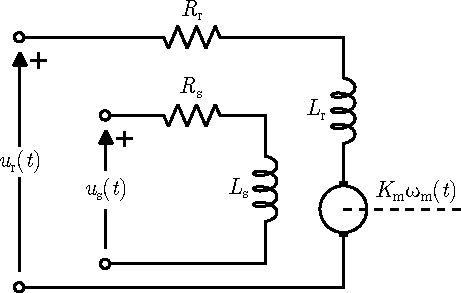
\includegraphics[width=0.9\textwidth]{fig/DCmotor.pdf}
        \caption{Model motora stalne struje.}
    \end{figure}
    \end{column}
\end{columns}
	
\end{frame}

%------------------------------------------------



\subsection{Rotacioni enkoder}

\begin{frame}{Rotacioni enkoder}
    \begin{figure}
    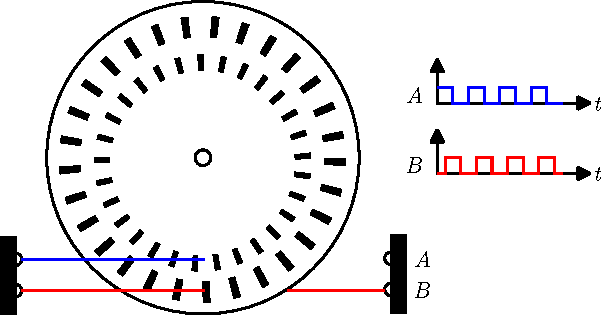
\includegraphics[width=0.6\linewidth]{fig/enc.pdf}
    \caption{Rotacioni enkoder.}
    \end{figure}
\end{frame}

%------------------------------------------------

\subsection{Pretvarač učestanosti u napon}

\begin{frame}{Pretvarač učestanosti u napon}
    \begin{figure}
    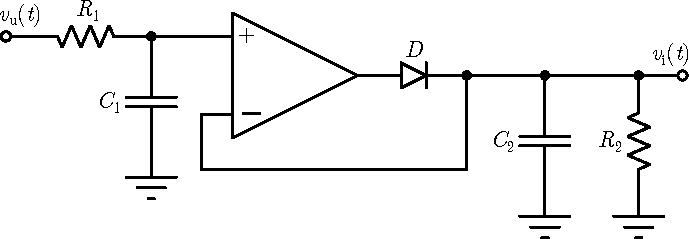
\includegraphics[width=0.6\linewidth]{fig/fv.pdf}
    \caption{Električna šema pretvarača učestanosti u napon.}
    \end{figure}
\end{frame}

%------------------------------------------------


\begin{frame}{Pretvarač učestanosti u napon}
    \begin{figure}
    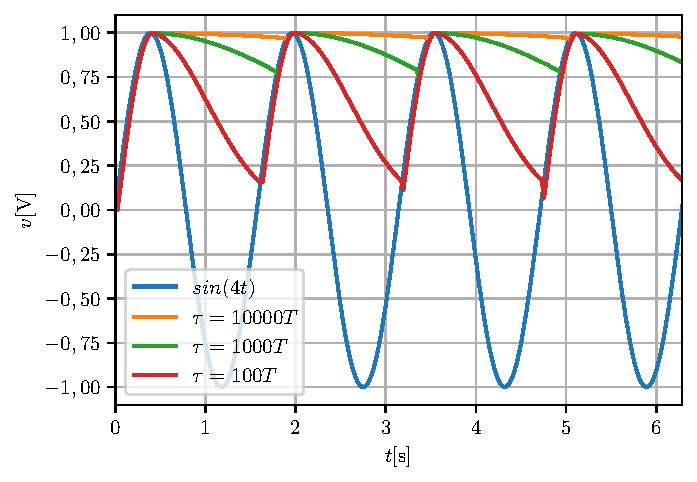
\includegraphics[width=0.6\linewidth]{fig/peakDet.pdf}
    \caption{Primer ulaznog signala i nekoliko izlaznih signala pretvarača učestanosti u napon.}
    \end{figure}
\end{frame}

%------------------------------------------------


\subsection{Negativna povratna sprega}

\begin{frame}{Negativna povratna sprega}
    \begin{figure}
    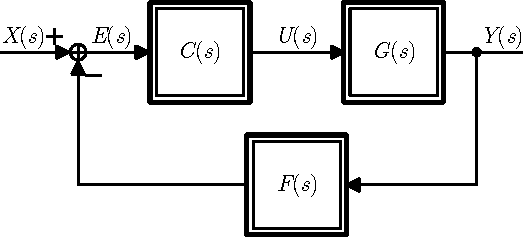
\includegraphics[width=0.6\linewidth]{fig/nps.pdf}
    \caption{Opšta blok šema sistema sa negativnom povratnom spregom.}
    \end{figure}
\end{frame}

%------------------------------------------------

\subsection{Regulatori}

\begin{frame}{P regulator}
    \begin{figure}
    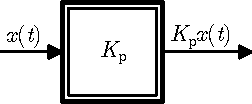
\includegraphics[width=0.3\linewidth]{fig/Preg.pdf}
    \caption{Opšta blok šema P regulatora.}
    \end{figure}
\end{frame}

%------------------------------------------------


\begin{frame}{Bang-bang regulator}
    
    
    \begin{columns}[c]
    \begin{column}{.25\textwidth}
    \centering
		\hfill    		 
    		 $K_{\rm p} \to \infty$   
    		 \hfill  
    \end{column}
    \begin{column}{.75\textwidth}
    \begin{figure}
    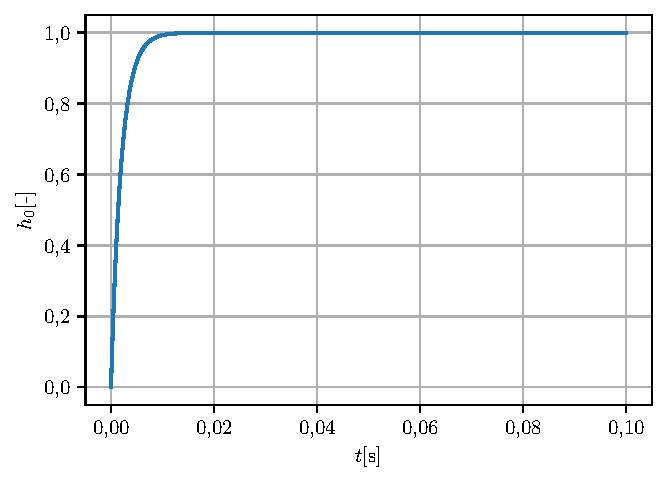
\includegraphics[width=0.7\linewidth]{fig/bbh.pdf}
    \caption{Očekivani napon na izlazu bang-bang regulatora.}
    \end{figure}
    \end{column}
\end{columns}
    
    
\end{frame}

%------------------------------------------------


\begin{frame}{PI regulator}
    \begin{figure}
    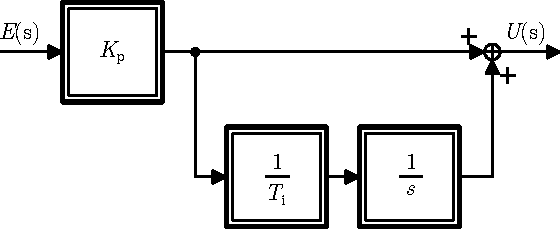
\includegraphics[width=0.6\linewidth]{fig/PIreg.pdf}
    \caption{Opšta blok šema sistema sa PI regulatorom.}
    \end{figure}
\end{frame}

%------------------------------------------------

\subsection{Pojačavači snage}

\begin{frame}{Pojačavači snage}
    \begin{figure}
    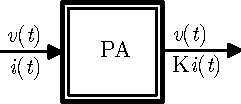
\includegraphics[width=0.3\linewidth]{fig/pa.pdf}
    \caption{Opšta blok šema sistema sa negativnom povratnom spregom.}
    \end{figure}
\end{frame}

%------------------------------------------------


\begin{frame}{Pojačavač snage u klasi B}
	\begin{columns}[c]
    \begin{column}{.5\textwidth}
    \begin{figure}
        \centering
        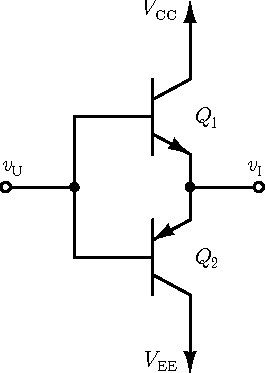
\includegraphics[scale = 0.75]{fig/PAB.pdf}
        \caption{Pojačavač snage u klasi B.}
    \end{figure}      
    \end{column}
    \begin{column}{.5\textwidth}
    \begin{figure}
        \centering
        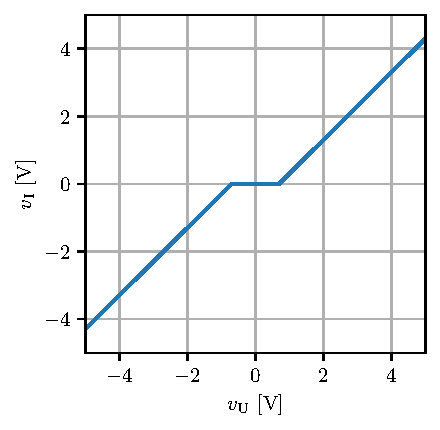
\includegraphics[width=0.65\textwidth]{fig/PAbkka.pdf}
        \caption{Jednosmerna prenosna karakteristika.}
    \end{figure}
    \end{column}
\end{columns}
\end{frame}

%------------------------------------------------


\begin{frame}{Pojačavač snage u klasi AB}
	\begin{columns}[c]
    \begin{column}{.5\textwidth}
    \begin{figure}
        \centering
        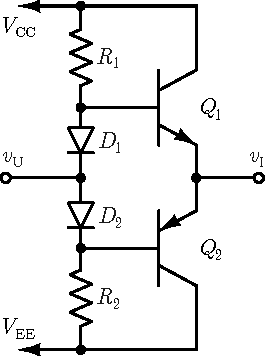
\includegraphics[scale = 0.75]{fig/PAAB.pdf}
        \caption{Pojačavač snage u klasi B.}
    \end{figure}      
    \end{column}
    \begin{column}{.5\textwidth}
    \begin{figure}
        \centering
        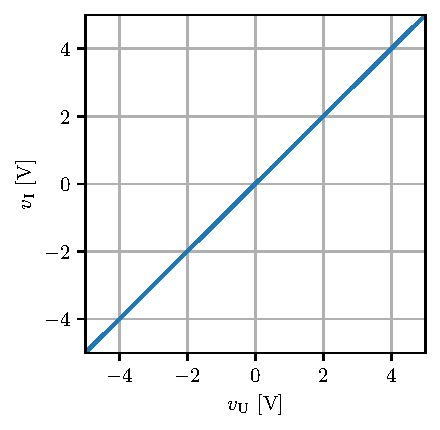
\includegraphics[width=0.65\textwidth]{fig/PAABkka.pdf}
        \caption{Jednosmerna prenosna karakteristika.}
    \end{figure}
    \end{column}
\end{columns}
\end{frame}

%------------------------------------------------

\section{Karakteristike korišćenih komponenti}

\begin{frame}
    \Huge{\centerline{\textbf{Karakteristike korišćenih komponenti}}}
\end{frame}
%------------------------------------------------

\subsection{Merenje karakteristike motora}

\begin{frame}{Merenje karakteristike motora}
	\begin{columns}[c]
    \begin{column}{.4\textwidth}
    \begin{figure}
        \centering
        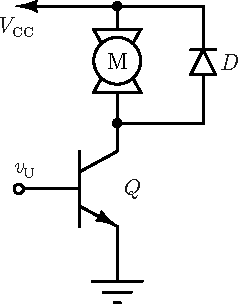
\includegraphics[scale = 0.75]{fig/DCtransistor.pdf}
        \caption{Električna šema za testiranje motora.}
    \end{figure}      
    \end{column}
    \begin{column}{.6\textwidth}
    \begin{figure}
        \centering
        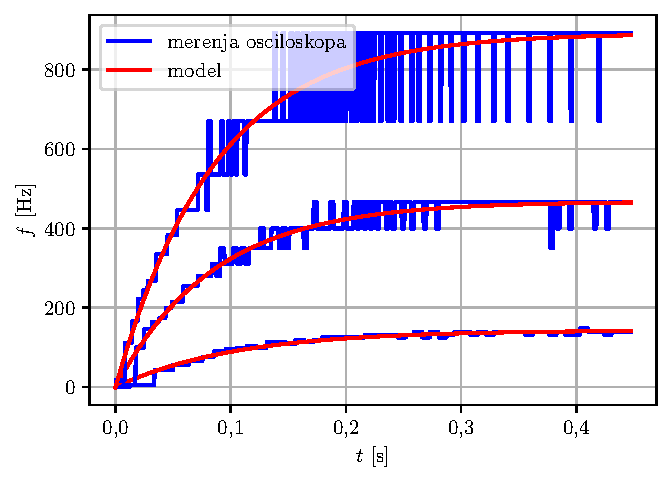
\includegraphics[width=0.75\textwidth]{fig/compact.pdf}
        \caption{Grafik preklopljenih izmerenih i modela karakteristike motora.}
    \end{figure}
    \end{column}
\end{columns}
\end{frame}

%------------------------------------------------


\begin{frame}{Greška merenja}
	\begin{columns}[c]
    \begin{column}{.4\textwidth}
    \centering
    		$$\frac{\Delta f}{f} = \frac{f \Delta t}{1 - (f \Delta f)^2}$$      
    \end{column}
    \begin{column}{.6\textwidth}
    \begin{figure}
        \centering
        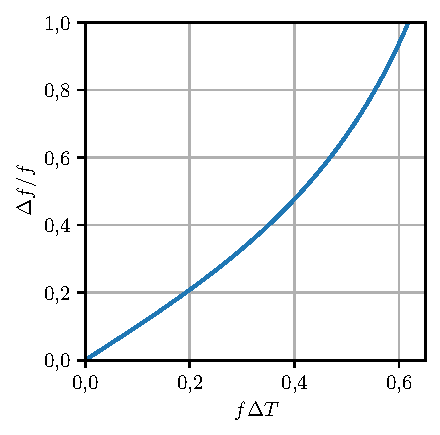
\includegraphics[width=0.65\textwidth]{fig/fGreska.pdf}
        \caption{Odnos normalizovane relativne greške u odnosu na normalizovanu frekvenciju.}
    \end{figure}
    \end{column}
\end{columns}
\end{frame}

%------------------------------------------------

\subsection{Pretvarač učestanosti u napon}

\begin{frame}{Pretvarač učestanosti u napon}
	\begin{columns}[c]
    \begin{column}{.5\textwidth}
    \begin{figure}
        \centering
        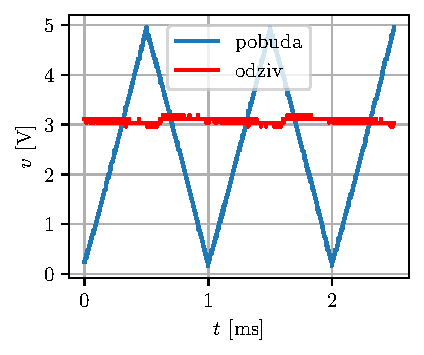
\includegraphics[scale = 0.75]{fig/FV1000s.pdf}
        \caption{Odziv pretvarača na pobudu konstante frekvencije.}
    \end{figure}      
    \end{column}
    \begin{column}{.5\textwidth}
    \begin{figure}
        \centering
        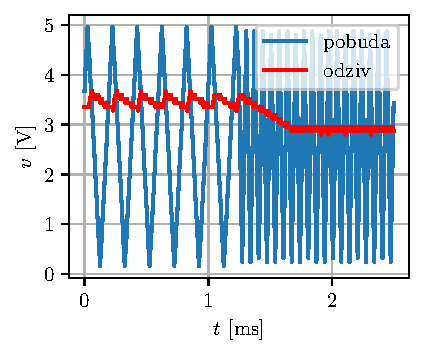
\includegraphics[width=0.75\textwidth]{fig/FV1000d.pdf}
        \caption{Odziv pretvarača na skokovitu promenu frekvencije pobudnog napona.}
    \end{figure}
    \end{column}
\end{columns}
\end{frame}

%------------------------------------------------

\begin{frame}{Pretvarač učestanosti u napon sa filtrom}
	\begin{columns}[c]
    \begin{column}{.5\textwidth}
    \begin{figure}
        \centering
        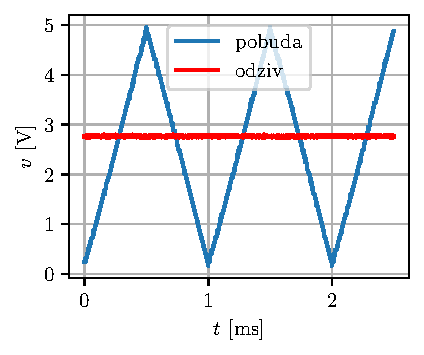
\includegraphics[scale = 0.75]{fig/FV1000sNF.pdf}
        \caption{Odziv pretvarača na pobudu konstante frekvencije.}
    \end{figure}      
    \end{column}
    \begin{column}{.5\textwidth}
    \begin{figure}
        \centering
        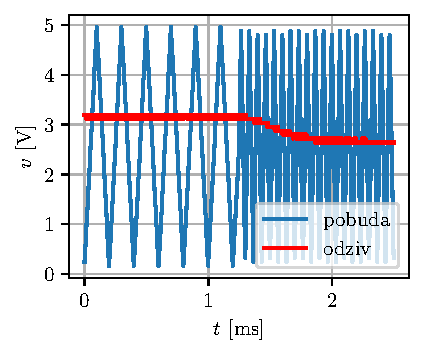
\includegraphics[width=0.75\textwidth]{fig/FV1000dNF.pdf}
        \caption{Odziv pretvarača na skokovitu promenu frekvencije pobudnog napona.}
    \end{figure}
    \end{column}
\end{columns}
\end{frame}

%------------------------------------------------

\begin{frame}{Karakteristika pretvarača frekvencije u napon}
    \begin{figure}
    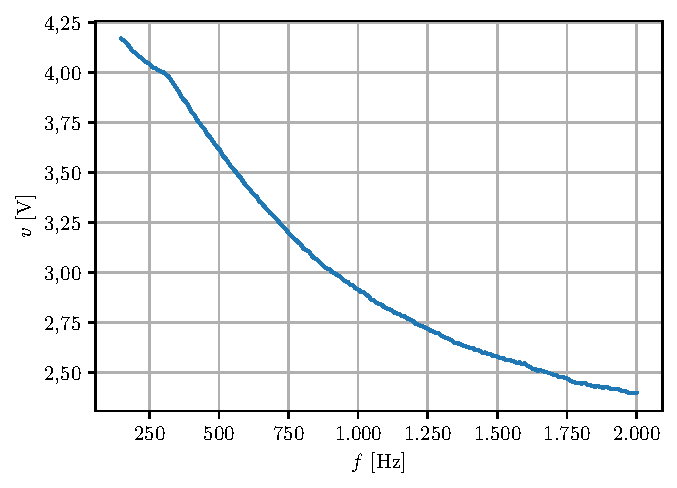
\includegraphics[width=0.6\linewidth]{fig/FVkka.pdf}
    \caption{Prenosna karakteristika pretvarača učestanosti.}
    \end{figure}
\end{frame}

%------------------------------------------------

\subsection{Karakteristike pojačavača snage}

\begin{frame}{Karakteristike pojačavača snage}
	\begin{columns}[c]
    \begin{column}{.5\textwidth}
    \begin{figure}
        \centering
        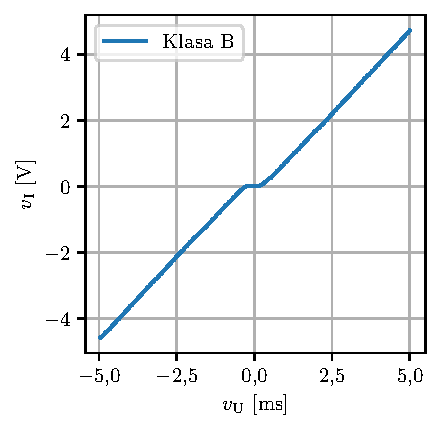
\includegraphics[scale = 0.75]{fig/PABs.pdf}
        \caption{Izmerena statička karakteristika pojačavača snage u klasi B.}
    \end{figure}      
    \end{column}
    \begin{column}{.5\textwidth}
    \begin{figure}
        \centering
        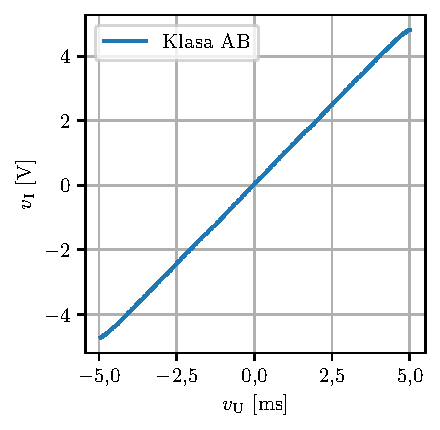
\includegraphics[width=0.75\textwidth]{fig/PAABs.pdf}
        \caption{Izmerena statička karakteristika pojačavača snage u klasi AB.}
    \end{figure}
    \end{column}
\end{columns}
\end{frame}

%------------------------------------------------

\begin{frame}{Karakteristike pojačavača snage}
	\begin{columns}[c]
    \begin{column}{.5\textwidth}
    \begin{figure}
        \centering
        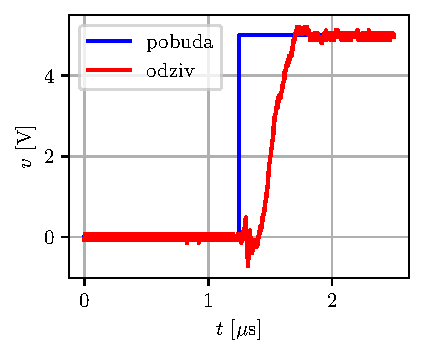
\includegraphics[scale = 0.75]{fig/PAstep.pdf}
        \caption{Izmeren odziv pojačavača u klasi AB na odskočnu pobudu.}
    \end{figure}      
    \end{column}
    \begin{column}{.5\textwidth}
    \begin{figure}
        \centering
        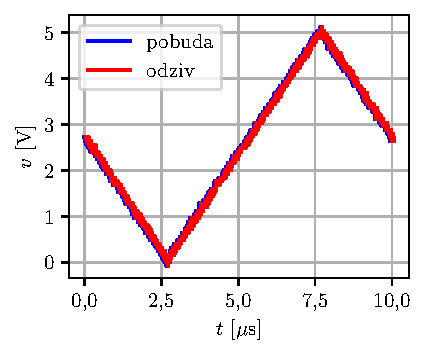
\includegraphics[width=0.75\textwidth]{fig/PAramp.pdf}
        \caption{Izmeren odziv pojačavača u klasi AB na rampu.}
    \end{figure}
    \end{column}
\end{columns}
\end{frame}

%------------------------------------------------

\begin{frame}{Kompletan sistem}
    \begin{figure}
    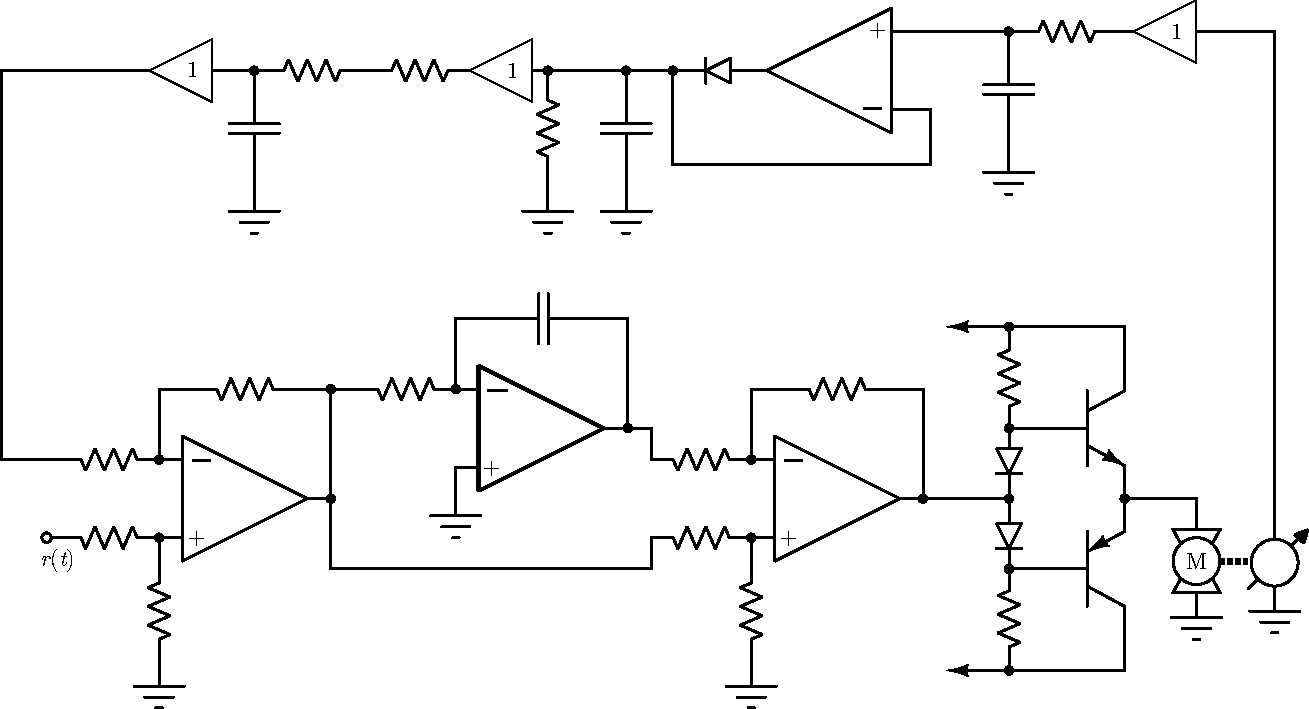
\includegraphics[width=0.75\linewidth]{fig/elFull.pdf}
    \caption{Blok šema celog sistema.}
    \end{figure}
\end{frame}

%------------------------------------------------

\begin{frame}{Radno merno okruženje}
    \begin{figure}
    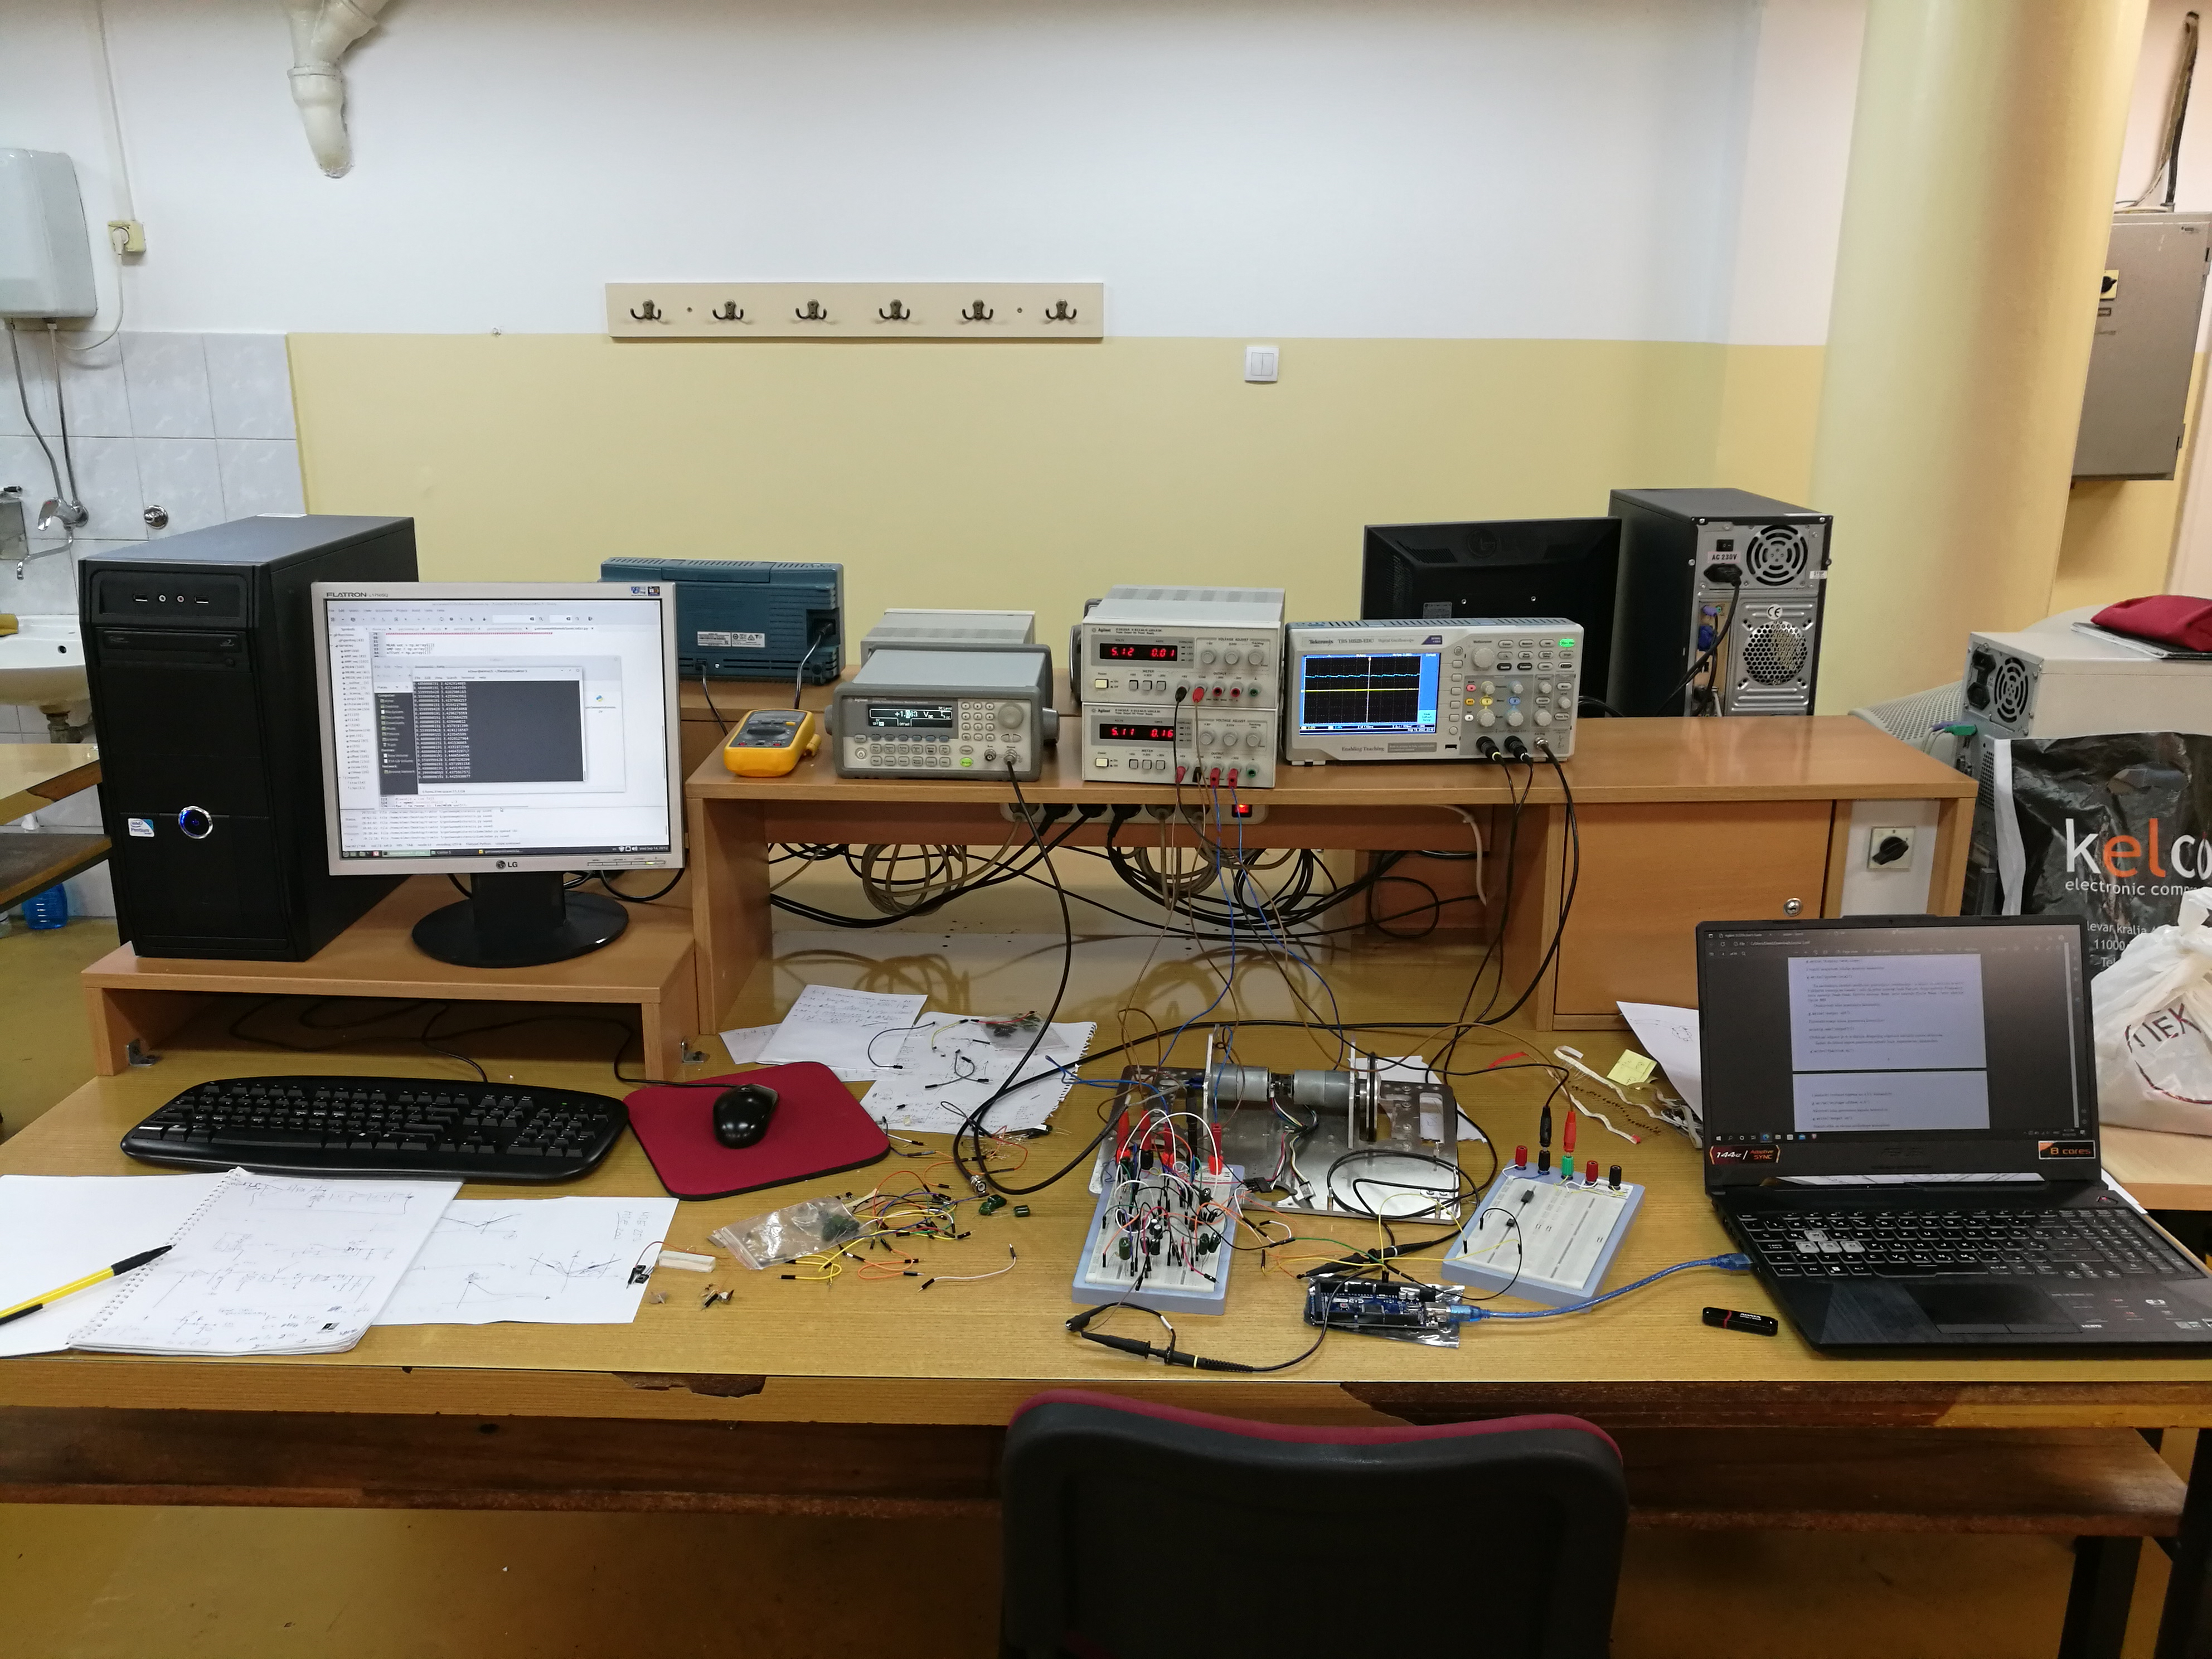
\includegraphics[width=0.6\linewidth]{fig/img/lab.jpg}
    \caption{Radno okruženje sa projektovanim sistemom i aparaturom za merenje.}
    \end{figure}
\end{frame}

%------------------------------------------------

\section{Rezultati i diskusija}

\begin{frame}
    \Huge{\centerline{\textbf{Rezultati i diskusija}}}
\end{frame}

%------------------------------------------------


\begin{frame}{Rezultati merenja karakteristike motora}
	\begin{columns}[c]
    \begin{column}{.3\textwidth}
    \begin{figure}
        \centering
        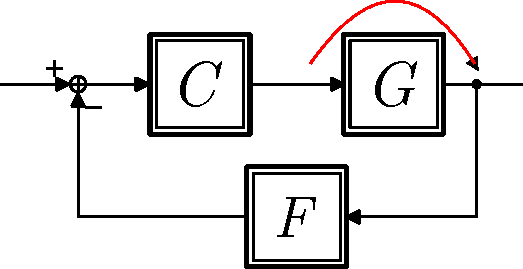
\includegraphics[scale = 0.5]{h/Hmotor1.pdf}
        \caption{Blok šema.}
    \end{figure}      
    \end{column}
    \begin{column}{.7\textwidth}
    \begin{figure}
        \centering
        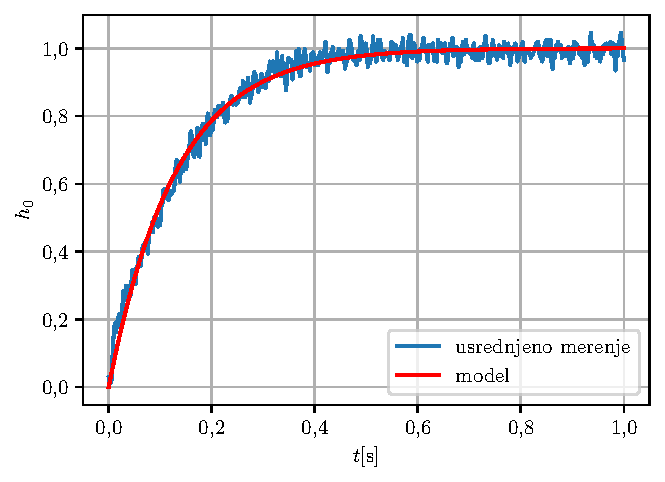
\includegraphics[width=0.75\textwidth]{fig/pi/Hsrednje.pdf}
        \caption{Usrednjeni relativni odziv sistema i njegov model sa parametrima $K_{\rm m} = 0.314$ i $T_{\rm m} = 132 \, \rm{ms}$.}
    \end{figure}
    \end{column}
\end{columns}
\end{frame}


%------------------------------------------------



\begin{frame}{Pozicije nule i polova sistema}
	\begin{columns}[c]
    \begin{column}{.5\textwidth}
    \begin{figure}
        \centering
        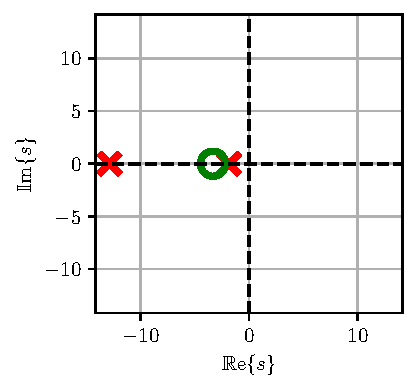
\includegraphics[scale = 0.75]{fig/zplane/BezPreskok.pdf}
        \caption{Pozicija nula i polova prenosne funkcije za sistem bez preskoka.}
    \end{figure}      
    \end{column}
    \begin{column}{.5\textwidth}
    \begin{figure}
        \centering
        \includegraphics[width=0.75\textwidth]{fig/zplane/preskok.pdf}
        \caption{Pozicija nula i polova prenosne funkcije za sistem sa preskokom.}
    \end{figure}
    \end{column}
\end{columns}
\end{frame}

%------------------------------------------------


\begin{frame}{Rezultati merenja sistema}
	\begin{columns}[c]
    \begin{column}{.3\textwidth}
    \begin{figure}
        \centering
        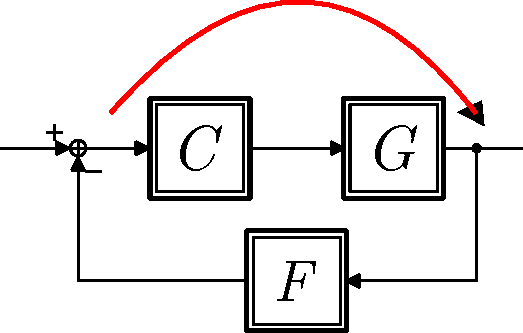
\includegraphics[scale = 0.5]{h/Hsis.pdf}
        \caption{Blok šema.}
    \end{figure}      
    \end{column}
    \begin{column}{.7\textwidth}
    \begin{figure}
        \centering
        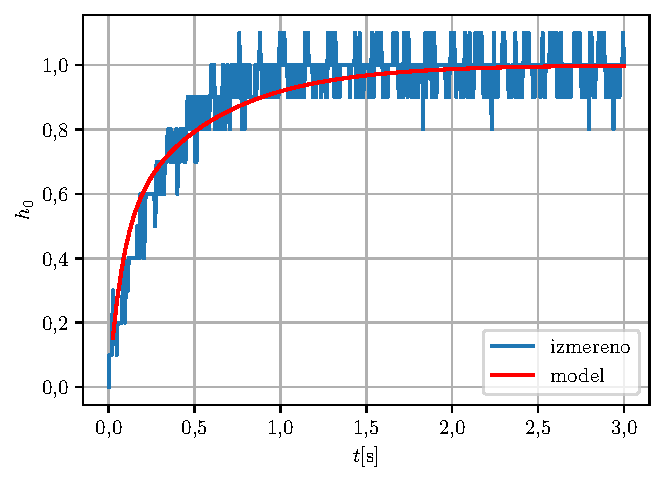
\includegraphics[width=0.75\textwidth]{fig/pi/k3t100.pdf}
        \caption{Odskočni odziv sistema sa parametrima PI regulatora  $K_{\rm p} = 3$ i $T_{\rm i} = 100 \, \rm{ms}$.}
    \end{figure}
    \end{column}
\end{columns}
\end{frame}


%------------------------------------------------

\begin{frame}{Rezultati merenja sistema}
	\begin{columns}[c]
    \begin{column}{.3\textwidth}
    \begin{figure}
        \centering
        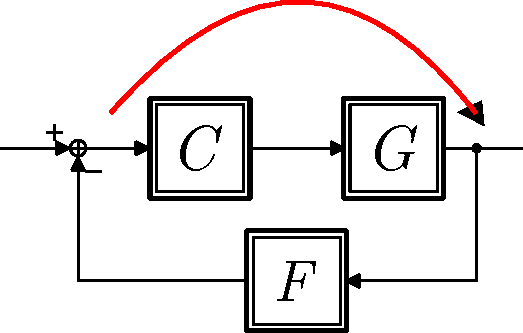
\includegraphics[scale = 0.5]{h/Hsis.pdf}
        \caption{Blok šema.}
    \end{figure}      
    \end{column}
    \begin{column}{.7\textwidth}
    \begin{figure}
        \centering
        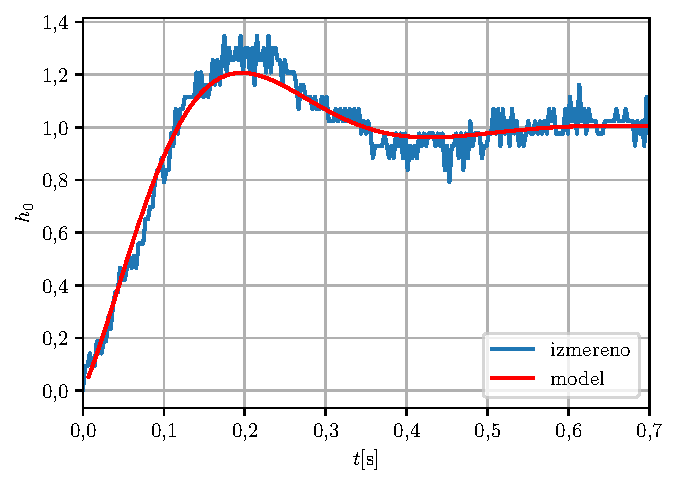
\includegraphics[width=0.75\textwidth]{fig/pi/k3t10.pdf}
        \caption{Odskočni odziv sistema sa parametrima PI regulatora  $K_{\rm p} = 3$ i $T_{\rm i} = 10 \, \rm{ms}$.}
    \end{figure}
    \end{column}
\end{columns}
\end{frame}

%------------------------------------------------

\begin{frame}{Zaključak}

	\begin{itemize}
		\item Teorija - modeli - merenja
		\item Preporuke za dalje modifikacije
			\begin{itemize}
				\item Model motora
				\item Smer okretanja
				\item FV pretvarač
				\item Hlađenje
			\end{itemize}
		
	\end{itemize}
    
\end{frame}



\begin{frame}

	\Huge{{\centerline{\textbf{Zahvalnost}}}}
    
\end{frame}


\begin{frame}

	\Huge{{\centerline{\textbf{Hvala na pažnji!}}}}
    
\end{frame}

%------------------------------------------------



%----------------------------------------------------------------------------------------

\end{document}